\documentclass[11pt]{article}

% ----- lightweight preamble (matches the other picture books in this project) -----
\usepackage[a4paper,margin=1.5cm]{geometry}
\usepackage{amsmath,amssymb}
\usepackage{booktabs}
\usepackage{tikz}
\usepackage{tikz-cd}
\usetikzlibrary{arrows.meta,positioning,calc,fit,backgrounds,
  shapes.geometric,chains,decorations.pathreplacing,decorations.markings}
\usepackage[most]{tcolorbox}
\usepackage{parskip}
\usepackage{xcolor}

\definecolor{ink}{RGB}{40,40,40}
\definecolor{soft}{RGB}{245,245,248}
\definecolor{gen}{RGB}{30,110,190}   % generic pattern  (TransitionSystem)
\definecolor{fib}{RGB}{30,140,80}    % Fibonacci / Cassini
\definecolor{crx}{RGB}{200,140,0}    % cross invariant / Frobenius
\definecolor{thm}{RGB}{130,70,170}   % categorical / trace
\definecolor{cic}{RGB}{170,60,60}    % CIC / Lean

% the four "gadget" badge colours used across this project's picture books
\definecolor{faceL}{RGB}{30,140,80}   % linearized trace  L
\definecolor{faceF}{RGB}{200,140,0}   % Frobenius / doubling  F
\definecolor{faceC}{RGB}{130,70,170}  % cyclotomic coset bookkeeping  C
\definecolor{faceX}{RGB}{30,110,190}  % categorical loop  X

\newtcolorbox{note}[1][]{colback=soft,colframe=ink,boxrule=0.4pt,
  arc=2pt,left=6pt,right=6pt,top=4pt,bottom=4pt,#1}
\newtcolorbox{verdict}[1][]{colback=fib!7,colframe=fib!65,boxrule=0.7pt,
  arc=2pt,left=7pt,right=7pt,top=5pt,bottom=5pt,#1}
\newtcolorbox{caveat}[1][]{colback=cic!6,colframe=cic!55,boxrule=0.6pt,
  arc=2pt,left=7pt,right=7pt,top=5pt,bottom=5pt,#1}

\tikzset{
  box/.style={draw=ink,rounded corners=3pt,fill=soft,inner sep=5pt,
    font=\small,align=center},
  code/.style={draw=ink,rounded corners=2pt,fill=white,inner sep=4pt,
    font=\ttfamily\scriptsize,align=left},
  arr/.style={-{Stealth[length=2.6mm]},thick},
  eq/.style={{Stealth[length=2.2mm]}-{Stealth[length=2.2mm]},thick,ink},
  lbl/.style={font=\scriptsize\itshape,text=ink,align=center},
  badge/.style={circle,inner sep=0pt,minimum size=3.8mm,font=\scriptsize\bfseries,text=white},
}
\newcommand{\bL}{\tikz[baseline=-0.6ex]\node[badge,fill=faceL]{L};}
\newcommand{\bF}{\tikz[baseline=-0.6ex]\node[badge,fill=faceF]{F};}
\newcommand{\bC}{\tikz[baseline=-0.6ex]\node[badge,fill=faceC]{C};}
\newcommand{\bX}{\tikz[baseline=-0.6ex]\node[badge,fill=faceX]{$\otimes$};}
\newcommand{\ck}{\textcolor{fib}{\checkmark}}
\newcommand{\lc}[1]{\texttt{\small #1}}

\title{\vspace{-1.6cm}\textbf{The same pattern, five costumes}\\[3pt]
\large Fibonacci, the gadgets \bL\,\bF\,\bC, and the categorical trace \bX\ ---
all one\\ model-checking invariant (\texttt{TransitionSystem} / \texttt{Reachable} / CIC)}
\author{\small Visual companion to
\texttt{RequestProject/ModelChecking/FibonacciTracePattern.lean}
(\lc{sorry}-free)}
\date{}

\begin{document}
\maketitle
\vspace{-1.1cm}

\begin{note}
\textbf{Your question.} The picture books say Theorem 6 has a \textbf{Fibonacci
pattern}, is built from the three \textbf{gadgets} \bL~linearized trace,
\bF~Frobenius, \bC~cyclotomic cosets, and from one \textbf{categorical gadget}
\bX~(the evaluation/coevaluation \emph{trace loop}, ``what returns''). \emph{Are
those same patterns already inside the model-checking core --- base/step,
\lc{Reachable}, \lc{TransitionSystem}, the cross invariant, and the CIC
reading?}

\smallskip
\textbf{Verified answer: yes.} Each one is literally an instance of a single
schema, and the accompanying Lean file proves it end to end, \lc{sorry}-free:
\begin{center}\itshape
base case holds \; $+$ \; every step preserves it
\;$\Longrightarrow$\; it holds at every reachable state.
\end{center}
That one theorem is \lc{ModelChecking.InductiveInvariant.reachable}; and (see
\texttt{CICLink.lean}) it \emph{is} CIC induction --- Lean's auto-generated
recursor \lc{Reachable.rec}. Below, every \ck\ box names a checked declaration.
\end{note}

%=====================================================================
\section*{0. The shared skeleton (proved once)}

\begin{center}
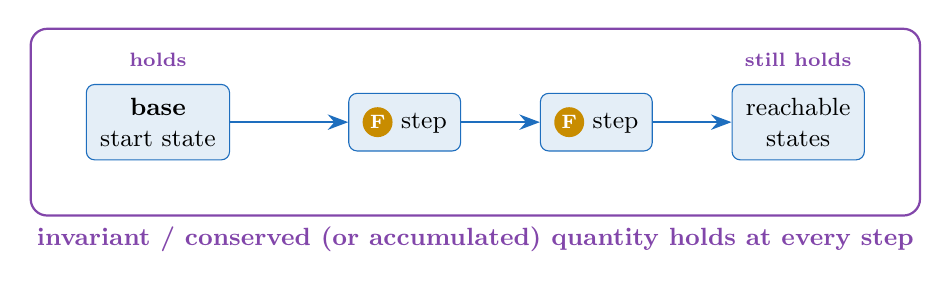
\begin{tikzpicture}[node distance=8mm]
  \node[box,fill=gen!12,draw=gen] (init) {\textbf{base}\\start state};
  \node[box,fill=gen!12,draw=gen,right=15mm of init] (s1) {\bF\ step};
  \node[box,fill=gen!12,draw=gen,right=10mm of s1] (s2) {\bF\ step};
  \node[box,fill=gen!12,draw=gen,right=10mm of s2] (s3) {reachable\\states};
  \draw[arr,gen] (init) -- (s1);
  \draw[arr,gen] (s1) -- (s2);
  \draw[arr,gen] (s2) -- (s3);
  \begin{scope}[on background layer]
    \node[fit=(init)(s3),draw=thm,thick,rounded corners=6pt,
      inner sep=7mm,label={[thm,font=\small\bfseries]below:%
      invariant / conserved (or accumulated) quantity holds at every step}] {};
  \end{scope}
  \node[thm,font=\scriptsize\bfseries,above=1mm of init] {holds};
  \node[thm,font=\scriptsize\bfseries,above=1mm of s3] {still holds};
\end{tikzpicture}
\end{center}

\begin{center}\footnotesize
\lc{TransitionSystem} $=$ (\lc{init}, \lc{step}); \;
\lc{Reachable} $=$ base $+$ step (a CIC \lc{inductive}); \;
\lc{InductiveInvariant} $=$ (\lc{init\_holds}, \lc{step\_preserves}); \;
soundness $=$ \lc{InductiveInvariant.reachable}.
\end{center}

%=====================================================================
\section*{1. The five costumes, side by side}

\begin{center}
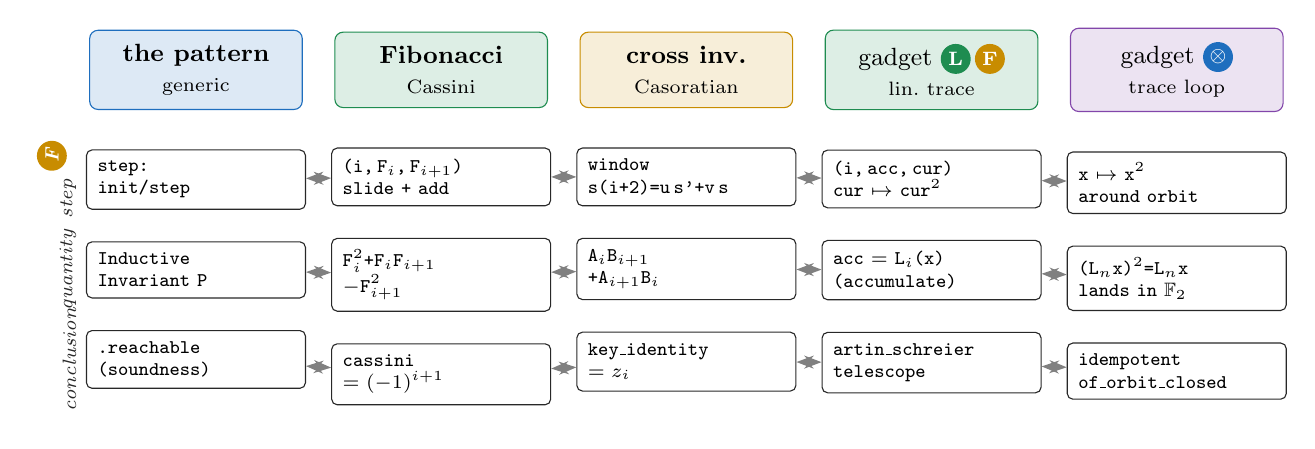
\begin{tikzpicture}[node distance=3mm]
  % headers
  \node[box,fill=gen!15,draw=gen,minimum width=27mm] (h0) {\textbf{the pattern}\\\scriptsize generic};
  \node[box,fill=fib!15,draw=fib,minimum width=27mm,right=4mm of h0] (h1) {\textbf{Fibonacci}\\\scriptsize Cassini};
  \node[box,fill=crx!15,draw=crx,minimum width=27mm,right=4mm of h1] (h2) {\textbf{cross inv.}\\\scriptsize Casoratian};
  \node[box,fill=faceL!15,draw=faceL,minimum width=27mm,right=4mm of h2] (h3) {gadget \bL\,\bF\\\scriptsize lin.\ trace};
  \node[box,fill=thm!15,draw=thm,minimum width=27mm,right=4mm of h3] (h4) {gadget \bX\\\scriptsize trace loop};

  % row: the machine / step
  \node[code,below=5mm of h0.south,anchor=north,text width=25mm] (c0) {step:\\ init/step};
  \node[code,below=5mm of h1.south,anchor=north,text width=25mm] (c1) {(i,\,F$_i$,\,F$_{i+1}$)\\ slide + add};
  \node[code,below=5mm of h2.south,anchor=north,text width=25mm] (c2) {window\\ s(i{+}2)=u\,s'{+}v\,s};
  \node[code,below=5mm of h3.south,anchor=north,text width=25mm] (c3) {(i,\,acc,\,cur)\\ cur $\mapsto$ cur$^2$};
  \node[code,below=5mm of h4.south,anchor=north,text width=25mm] (c4) {x $\mapsto$ x$^2$\\ around orbit};
  \node[lbl,left=0mm of c0,rotate=90,anchor=south] {step \bF};

  % row: the tracked quantity
  \node[code,below=4mm of c0.south,anchor=north,text width=25mm] (d0) {Inductive\\Invariant P};
  \node[code,below=4mm of c1.south,anchor=north,text width=25mm] (d1) {F$_i^2$+F$_i$F$_{i+1}$\\ $-$F$_{i+1}^2$};
  \node[code,below=4mm of c2.south,anchor=north,text width=25mm] (d2) {A$_i$B$_{i+1}$\\ +A$_{i+1}$B$_i$};
  \node[code,below=4mm of c3.south,anchor=north,text width=25mm] (d3) {acc $=$ L$_i$(x)\\ (accumulate)};
  \node[code,below=4mm of c4.south,anchor=north,text width=25mm] (d4) {(L$_n$x)$^2$=L$_n$x\\ lands in $\mathbb F_2$};
  \node[lbl,left=0mm of d0,rotate=90,anchor=south] {quantity};

  % row: the conclusion (one theorem)
  \node[code,below=4mm of d0.south,anchor=north,text width=25mm] (e0) {.reachable\\ (soundness)};
  \node[code,below=4mm of d1.south,anchor=north,text width=25mm] (e1) {cassini\\ $=(-1)^{i+1}$};
  \node[code,below=4mm of d2.south,anchor=north,text width=25mm] (e2) {key\_identity\\ $=z_i$};
  \node[code,below=4mm of d3.south,anchor=north,text width=25mm] (e3) {artin\_schreier\\ telescope};
  \node[code,below=4mm of d4.south,anchor=north,text width=25mm] (e4) {idempotent\\ of\_orbit\_closed};
  \node[lbl,left=0mm of e0,rotate=90,anchor=south] {conclusion};

  \foreach \a/\b in {c0/c1,c1/c2,c2/c3,c3/c4,d0/d1,d1/d2,d2/d3,d3/d4,e0/e1,e1/e2,e2/e3,e3/e4}
    \draw[eq,gray] (\a) -- (\b);
\end{tikzpicture}
\end{center}

\begin{center}\footnotesize
\textcolor{gray}{$\longleftrightarrow$ each grey link $=$ ``same shape, different
words''.}\quad All boxes \ck\ in \lc{FibonacciTracePattern.lean}.
\end{center}

%=====================================================================
\section*{2. The Fibonacci pattern \emph{is} a transition system; Cassini \emph{is} a cross invariant}

The two-step recurrence $F_{i+2}=F_{i+1}+F_i$ is a \lc{TransitionSystem} on the
window $(i,F_i,F_{i+1})$. Cassini's identity is the \emph{sign-alternating}
inductive invariant --- the Fibonacci twin of Theorem 6's Casoratian.

\begin{center}
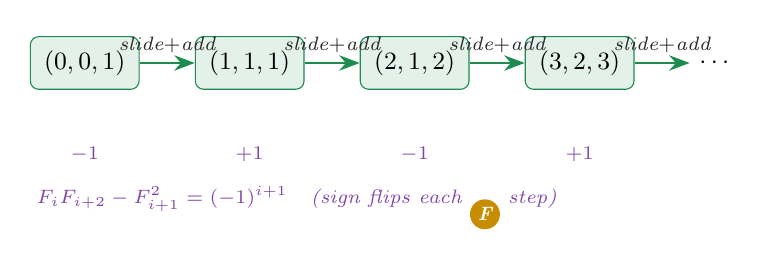
\begin{tikzpicture}[start chain=going right,node distance=7mm]
  \node[on chain,box,fill=fib!12,draw=fib] (r0) {$(0,0,1)$};
  \node[on chain,box,fill=fib!12,draw=fib] (r1) {$(1,1,1)$};
  \node[on chain,box,fill=fib!12,draw=fib] (r2) {$(2,1,2)$};
  \node[on chain,box,fill=fib!12,draw=fib] (r3) {$(3,2,3)$};
  \node[on chain,font=\small] (rd) {$\cdots$};
  \foreach \a/\b in {r0/r1,r1/r2,r2/r3,r3/rd}
    \draw[arr,fib] (\a) -- node[lbl,above]{slide$+$add} (\b);
  \node[thm,font=\scriptsize,below=6mm of r0] {$-1$};
  \node[thm,font=\scriptsize,below=6mm of r1] {$+1$};
  \node[thm,font=\scriptsize,below=6mm of r2] {$-1$};
  \node[thm,font=\scriptsize,below=6mm of r3] {$+1$};
  \node[lbl,thm,below=11mm of r1,xshift=6mm]
    {$F_iF_{i+2}-F_{i+1}^2=(-1)^{i+1}$ \; (sign flips each \bF\ step)};
\end{tikzpicture}
\end{center}

\begin{center}\footnotesize
\ck\ \lc{fibSystem}, \lc{fibWindow\_reachable}, \lc{cassiniInv},
\lc{cassini\_is\_inductiveInvariant}, \lc{cassini}. \; Kin:
\lc{CrossInvariant.lean} (\lc{key\_identity\_via\_reachable}),
\lc{Theorem6.lean} (\lc{casoratian}, \lc{cross\_invariant}).
\end{center}

%=====================================================================
\section*{3. The gadgets \bL\ and \bF: the linearized trace is a folded accumulator}

Frobenius \bF\ ($x\mapsto x^2$) is the \lc{step}. The linearized trace
\bL, $L_k(x)=\sum_{i<k}x^{2^i}$, is exactly the \emph{accumulator} carried along
the run --- so \bL\ is ``\bF\ folded''.

\begin{center}
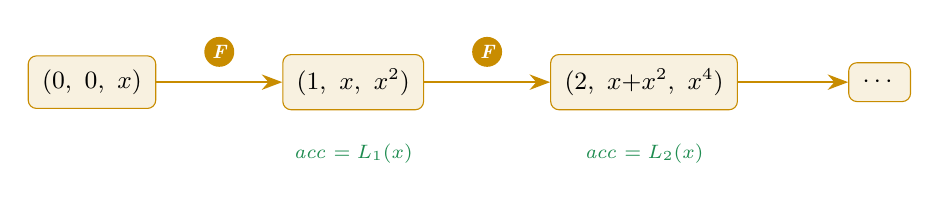
\begin{tikzpicture}[node distance=9mm]
  \node[box,fill=faceF!12,draw=faceF] (s0) {$(0,\ 0,\ x)$};
  \node[box,fill=faceF!12,draw=faceF,right=16mm of s0] (s1) {$(1,\ x,\ x^2)$};
  \node[box,fill=faceF!12,draw=faceF,right=16mm of s1] (s2) {$(2,\ x{+}x^2,\ x^4)$};
  \node[box,fill=faceF!12,draw=faceF,right=14mm of s2] (s3) {$\cdots$};
  \draw[arr,faceF] (s0) -- node[lbl,above]{\bF} (s1);
  \draw[arr,faceF] (s1) -- node[lbl,above]{\bF} (s2);
  \draw[arr,faceF] (s2) -- (s3);
  \node[lbl,below=3mm of s1,faceL] {acc $=L_1(x)$};
  \node[lbl,below=3mm of s2,faceL] {acc $=L_2(x)$};
\end{tikzpicture}
\end{center}

\begin{center}\small
The \bL--\bF\ glue (equation (1) of the paper), an invariant of the run:\quad
$L_k(x^2+x)=x^{2^k}+x$.
\end{center}
\begin{center}\footnotesize
\ck\ \lc{truncTrace}, \lc{traceSystem}, \lc{traceInv},
\lc{trace\_is\_inductiveInvariant}, \lc{traceWindow\_reachable},
\lc{truncTrace\_artin\_schreier}.
\end{center}

%=====================================================================
\section*{4. The categorical gadget \bX: ``what returns'' $=$ the loop closes}

The trace loop opens a wire (coevaluation), lets \bF\ walk the orbit, and closes
it (evaluation): what survives is the \emph{round trip}. When the Frobenius orbit
\emph{closes} ($x^{2^n}=x$), the accumulated trace becomes a fixed point of \bF\
--- it is idempotent, so it lands in the ground field $\mathbb F_2$: the
string-diagram slogan ``the closed loop returns to the unit object $I$''.

\begin{center}
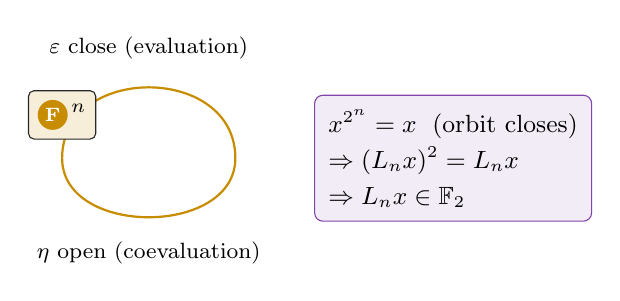
\begin{tikzpicture}[baseline]
  \draw[thick,faceF] (0,0) .. controls (0,-1) and (2.2,-1) .. (2.2,0);
  \draw[thick,faceF] (0,0) .. controls (0,1.2) and (2.2,1.2) .. (2.2,0);
  \node[draw=ink,fill=faceF!15,rounded corners=2pt,minimum size=6mm] at (0,0.55) {\bF$^{\,n}$};
  \node[font=\footnotesize] at (1.1,1.4) {$\varepsilon$ close (evaluation)};
  \node[font=\footnotesize] at (1.1,-1.2) {$\eta$ open (coevaluation)};
  \node[box,fill=thm!10,draw=thm,align=left,anchor=west] at (3.2,0)
    {$x^{2^n}=x$ \;(orbit closes)\\[2pt]
     $\Rightarrow (L_n x)^2=L_n x$\\[2pt]
     $\Rightarrow L_n x\in\mathbb F_2$};
\end{tikzpicture}
\end{center}

\begin{center}\footnotesize
\ck\ \lc{truncTrace\_frobenius} (\bF\ commutes with \bL),
\lc{truncTrace\_idempotent\_of\_orbit\_closed} (loop closes $\Rightarrow$ lands
in the base).
\end{center}

%=====================================================================
\section*{5. The gadget \bC: the survivors of the loop form a subgroup}

The fixed points of $\bF^k$ (the \emph{surviving loops} $=$ cyclotomic cosets,
gadget \bC) are closed under addition (freshman's dream): so ``what returns'' is
an additive subgroup --- exactly the coset bookkeeping \bC\ counts.

\begin{center}\footnotesize
\ck\ \lc{frob\_fixed\_closed\_add}:\quad
$x^{2^k}=x,\ y^{2^k}=y \;\Rightarrow\; (x+y)^{2^k}=x+y$.
\end{center}

%=====================================================================
\section*{6. Master table}

\begin{center}\scriptsize
\renewcommand{\arraystretch}{1.3}
\begin{tabular}{@{}p{2.9cm} p{2.3cm} p{4.0cm} p{5.8cm}@{}}
\toprule
\textbf{Paper pattern} & \textbf{Model-checking name} & \textbf{One shared idea} &
\textbf{Lean (\lc{...Pattern.lean})} \\
\midrule
Fibonacci recursion & \lc{Transition\allowbreak System} $+$ \lc{Reachable} &
  base $+$ two-step slide generates the run &
  \lc{fibSystem}, \lc{fibWindow\_reachable}\ \ck \\
Cassini identity & inductive invariant &
  quantity fixed (up to sign) by every step &
  \lc{cassini\_is\_inductiveInvariant}, \lc{cassini}\ \ck \\
cross invariant (Thm 6) & inductive invariant &
  Casoratian conserved: $=z_i$ at every $i$ &
  \lc{Cross\allowbreak Invariant.\allowbreak key\_\allowbreak identity\_\allowbreak via\_\allowbreak reachable}\ \ck \\
\bF\ Frobenius & \lc{step} &
  the next-state map $x\mapsto x^2$ &
  \lc{traceSystem}.\lc{step}\ \ck \\
\bL\ linearized trace & accumulated invariant &
  \lc{acc} folded along the \bF-run &
  \lc{trace\_is\_inductiveInvariant}\ \ck \\
\bC\ cyclotomic cosets & the reachable/return set &
  fixed points of $\bF^k$ (a subgroup) &
  \lc{frob\_fixed\_closed\_add}\ \ck \\
\bX\ categorical trace & \lc{Reachable} closes $=$ CIC recursor &
  ``what returns''; closed loop lands in $I$ &
  \lc{truncTrace\_\allowbreak idempotent\_\allowbreak of\_\allowbreak orbit\_\allowbreak closed}\ \ck \\
soundness & \lc{Inductive\-Invariant.\-reachable} & one theorem for all rows;
  it \emph{is} \lc{Reachable.rec} & \lc{CICLink.Inductive.reachable'}\ \ck \\
\bottomrule
\end{tabular}
\end{center}

%=====================================================================
\section*{7. Verdict}

\begin{verdict}
\textbf{Are the Fibonacci pattern, the gadgets \bL\,\bF\,\bC, and the categorical
trace \bX\ all present in the model-checking / CIC core?} Yes --- and it is now
machine-checked. Each is the single move \emph{base $+$ step $\Rightarrow$
reachable}: \bF\ is the \lc{step}; \bL\ is the accumulator folded along the run;
Fibonacci/Cassini and the Theorem-6 cross invariant are the conserved quantity;
\bC\ is the return/fixed-point set; and \bX, ``what returns'', is precisely the
\lc{Reachable} inductive closing on itself --- whose soundness \emph{is} the CIC
recursor \lc{Reachable.rec}. One theorem, \lc{InductiveInvariant.reachable},
discharges all of them.
\end{verdict}

\begin{caveat}
\textbf{A lens, not a magic wand.} The pattern unifies the \emph{shape} of these
devices and this file proves the shape end to end. It does not, by itself,
deliver the paper's genuinely extra mathematics --- the Fibonacci \emph{weight}
recursion $w(A_{i+2})=w(A_{i+1})+w(A_i)$ with $w(R)=2F_{k'}-1$, or the
Gau\ss/Jacobi-sum evaluation behind the difference sets. Those still need their
own arguments; the pattern says \emph{what to look at}, uniformly:
base, step, and what is conserved or returns.
\end{caveat}

\vfill
\begin{center}\footnotesize
Companion to \texttt{PatternMap.tex}, \texttt{CICLink.tex},
\texttt{Dobbertin\_OneCategoricalPattern.tex}, \texttt{PaperStory.tex}.\\
Source of every \ck: \texttt{RequestProject/ModelChecking/FibonacciTracePattern.lean}
(builds \lc{sorry}-free with \lc{lake build}).\\
Rebuild this document: \texttt{tectonic FibonacciPatternMap.tex}.
\end{center}

\end{document}
